%%%%%%%%%%%%%%%%%%%%%%%%%%%%%%%%%%%%%%%%%
% Journal Article
% LaTeX Template
% Version 1.4 (15/5/16)
%
% This template has been downloaded from:
% http://www.LaTeXTemplates.com
%
% Original author:
% Frits Wenneker (http://www.howtotex.com) with extensive modifications by
%  - Vel (vel@LaTeXTemplates.com)

%  - Alejandro M. Aragón (a.m.aragon@tudelft.nl)
%
% License:
% CC BY-NC-SA 3.0 (http://creativecommons.org/licenses/by-nc-sa/3.0/)
%
%%%%%%%%%%%%%%%%%%%%%%%%%%%%%%%%%%%%%%%%%

%----------------------------------------------------------------------------------------
%	PACKAGES AND OTHER DOCUMENT CONFIGURATIONS
%----------------------------------------------------------------------------------------

\documentclass[twoside,twocolumn,10pt]{article}

\usepackage{blindtext} % Package to generate dummy text throughout this template 

\usepackage[sc]{mathpazo} % Use the Palatino font
\usepackage[T1]{fontenc} % Use 8-bit encoding that has 256 glyphs
\linespread{1.05} % Line spacing - Palatino needs more space between lines
\usepackage{microtype} % Slightly tweak font spacing for aesthetics
\usepackage[english]{babel} % Language hyphenation and typographical rules
\usepackage{graphicx}
\usepackage{physics}
\usepackage{amsmath, amssymb}


\usepackage[hmarginratio=1:1,top=25mm,left=20mm,right=20mm,bottom=25mm,columnsep=20pt]{geometry} % Document margins
\usepackage[hang, small,labelfont=bf,up,textfont=it,up]{caption} % Custom captions under/above floats in tables or figures
\usepackage{booktabs} % Horizontal rules in tables

\usepackage{lettrine} % The lettrine is the first enlarged letter at the beginning of the text

\usepackage{enumitem} % Customized lists
\setlist[itemize]{noitemsep} % Make itemize lists more compact

\usepackage{abstract} % Allows abstract customization
\renewcommand{\abstractnamefont}{\normalfont\bfseries} % Set the "Abstract" text to bold
\renewcommand{\abstracttextfont}{\normalfont\small\itshape} % Set the abstract itself to small italic text

\usepackage{titlesec} % Allows customization of titles
\renewcommand\thesection{\Roman{section}} % Roman numerals for the sections
\renewcommand\thesubsection{\roman{subsection}} % roman numerals for subsections
\titleformat{\section}[block]{\large\scshape\centering}{\thesection.}{1em}{} % Change the look of the section titles
\titleformat{\subsection}[block]{\large}{\thesubsection.}{1em}{} % Change the look of the section titles

\usepackage{fancyhdr} % Headers and footers
\pagestyle{fancy} % All pages have headers and footers
\fancyhead{} % Blank out the default header
\fancyfoot{} % Blank out the default footer
\fancyhead[C]{Running title $\bullet$ May 2016 $\bullet$ Vol. XXI, No. 1} % Custom header text
\fancyfoot[RO,LE]{\thepage} % Custom footer text

\usepackage{titling} % Customizing the title section


\usepackage[dvipsnames, table]{xcolor}
\usepackage{booktabs}
\usepackage{tabularx}
\usepackage{multirow}
\usepackage{threeparttable}
\usepackage{subcaption}
\usepackage{listings}
\lstset{
  basicstyle=\ttfamily\small,  % 设置代码字体和大小
  numbers=left,                % 行号放在左侧
  breaklines=true, % 设置自动换行
  numberstyle=\tiny,          % 行号的字体大小
  keywordstyle=\color{blue},  % 关键字颜色
  commentstyle=\color{green}, % 注释颜色
  stringstyle=\color{red},    % 字符串颜色
  frame=single,               % 代码周围的框
  rulecolor=\color{black},    % 框的颜色
  xleftmargin=2em,            % 代码块左侧的边距
  captionpos=b                % 标题位置在底部
}

\usepackage{hyperref} % For hyperlinks in the PDF
\hypersetup{colorlinks=true, linkcolor=black, filecolor=black, urlcolor=black, citecolor=black}



\newcolumntype{L}[1]{>{\hsize=#1\hsize\raggedright
  \arraybackslash}X}
\newcolumntype{R}[1]{>{\hsize=#1\hsize\raggedleft
  \arraybackslash}X}
\newcolumntype{C}[2]{>{\hsize=#1\hsize\columncolor{#2}
  \centering\arraybackslash}X}
\newcommand{\ra}[1]{\renewcommand{\arraystretch}{#1}}
\newcommand{\scell}[2]{\cellcolor{#2} #1 }


\usepackage{pgfplots}
\usetikzlibrary{calc}
\usepgfplotslibrary{colorbrewer}


%----------------------------------------------------------------------------------------
%	TITLE SECTION
%----------------------------------------------------------------------------------------

\setlength{\droptitle}{-6\baselineskip} % Move the title up

\pretitle{\begin{center}\Huge\bfseries} % Article title formatting
\posttitle{\end{center}} % Article title closing formatting
\title{Final Project for Advanced FEM (ME46050)} % Article title
\author{%
\textsc{Xusen Qin} \\[1ex] % Your name
\normalsize Student ID: 5594979, email \href{X.Qin-2@student.tudelft.nl}{X.Qin-2@student.tudelft.nl}, % Your email address
edition: 2022-2023
}
\date{} % Leave empty to omit a date
\renewcommand{\maketitlehookd}{%
%\begin{abstract}
%\noindent \blindtext % Dummy abstract text - replace \blindtext with your abstract text
%\end{abstract}
}

%----------------------------------------------------------------------------------------

\begin{document}

% Print the title
\maketitle

%----------------------------------------------------------------------------------------
%	ARTICLE CONTENTS
%----------------------------------------------------------------------------------------

\section{Introduction}

\lettrine[nindent=0em,lines=3]{T}his report addresses two advanced finite element problems. The first problem constructs a solver for a one-dimensional Poisson equation using both h-version and p-version finite elements. The second problem develops a solver for a two-dimensional stress distribution of elliptical inhomogeneity in plane elasticity, employing the h-version FEM with T3 element and Q4 elements.


\section{\textbf{PRMBLEM 1}}
\subsection{Question 1}

The code for finite element method, shape functions as well as the gaussion integration method in Appendix.\ref{Apdx:FEM_1D}, \ref{Apdx:shape_1D}, and \ref{Apdx:Gaussian-1D}.

\begin{figure}[htbp]
  \centering
  \begin{subfigure}[b]{0.32\textwidth}
    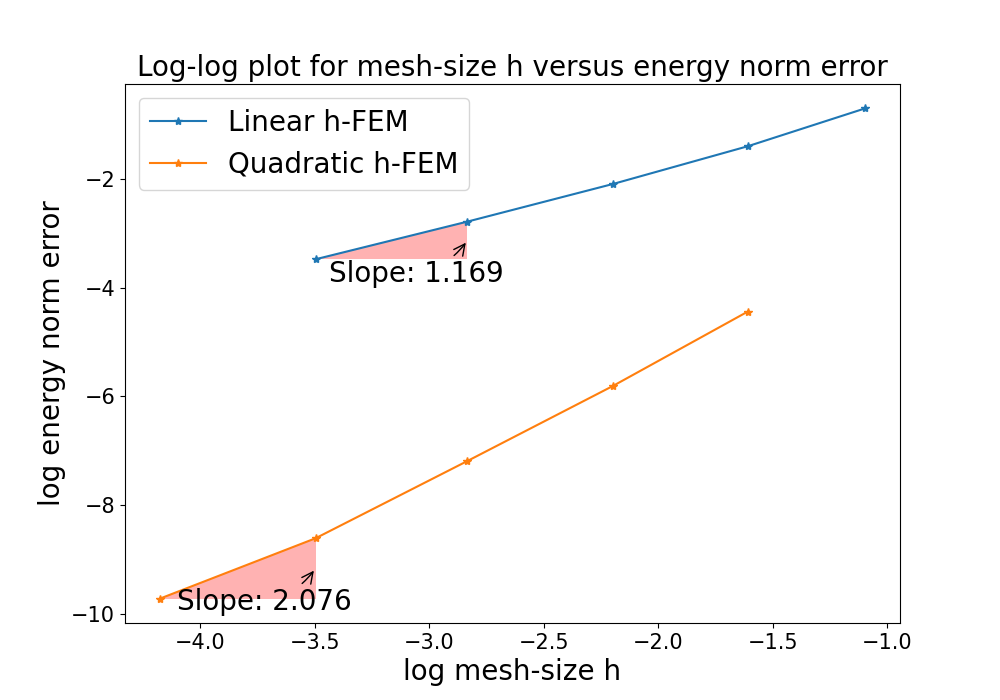
\includegraphics[width=1.\linewidth]{Q1/logmeshsize.png}
    \caption{log-log plot for the error versus meshsize}
    \label{fig:logmeshsize}
  \end{subfigure}
  % \hfill
  \begin{subfigure}[b]{0.32\textwidth}
    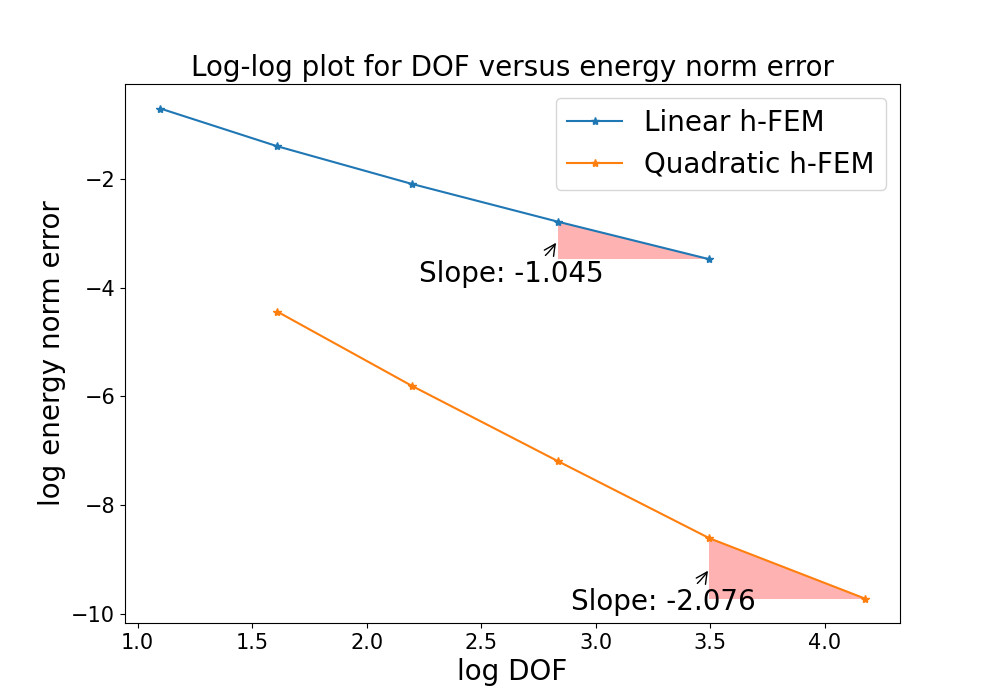
\includegraphics[width=1.\linewidth]{Q1/logDOF.png}
    \caption{log-log plot for the error versus DOF}
    \label{fig:logDOF}
  \end{subfigure}
\caption{The log-log figure for the energy norm error versus mesh size and DOF.}
\label{fig:Q1_1}
\end{figure}

The precise strain energy for this problem is given as U=0.03559183822564316. To determine the rates of convergence in the energy norm for both element types, we focus on terminal convergence by considering the last two points in the convergence plots.

The formula for the convergence rate can be found in Eq.\ref{eq:rate}, which can also be defined as the slope of the log-log plot. For both elements, the error decreases with the increase of the DOFs and the decrease of the mesh size. It's noteworthy that the convergence rate for the quadratic elements is approximately greater than that for the linear elements. Given the smoothness of the solution, the theoretical rates of convergence are typically 2 for linear elements and 4 for quadratic elements. For the computed errors, the linear elements exhibit an error of approximately \(0.031\), while the quadratic elements have a significantly smaller error of about \(6.0 \times 10^{-5}\). These computed rates align closely with the theoretical expectations.

\begin{equation}
\text{Rate} = \frac{\log(\text{error}_2) - \log(\text{error}_1)}{\log(\text{DOF}_2) - \log(\text{DOF}_1)}
\label{eq:rate}
\end{equation}

\subsection{Question 2}
In the log-log plot in Fig.\ref{fig:h_p_error} of the relative error in the energy norm versus the number of DOFs, the slopes of the plotted lines represent these rates. The inclusion of h-version plots in the same figure provides a comparative perspective, showcasing the efficiency and accuracy of each method relative to the other.

Given the computed convergence rates for the different finite element methods, we observe the following rates:
\begin{itemize}
    \item For Linear h-FEM: The rate of convergence is approximately -1.045.
    \item For Quadratic h-FEM: The rate of convergence is approximately -2.076.
    \item For p-FEM: The rate of convergence is approximately -8.245.
\end{itemize}
The negative values for the convergence rates indicate that the error decreases as the number of DOFs increases, which is expected in a convergence study. From the rates, it's evident that the p-FEM has the steepest convergence, indicating a faster reduction in error with increasing DOFs compared to the other methods. 

\begin{figure}[!ht]
  \centering
  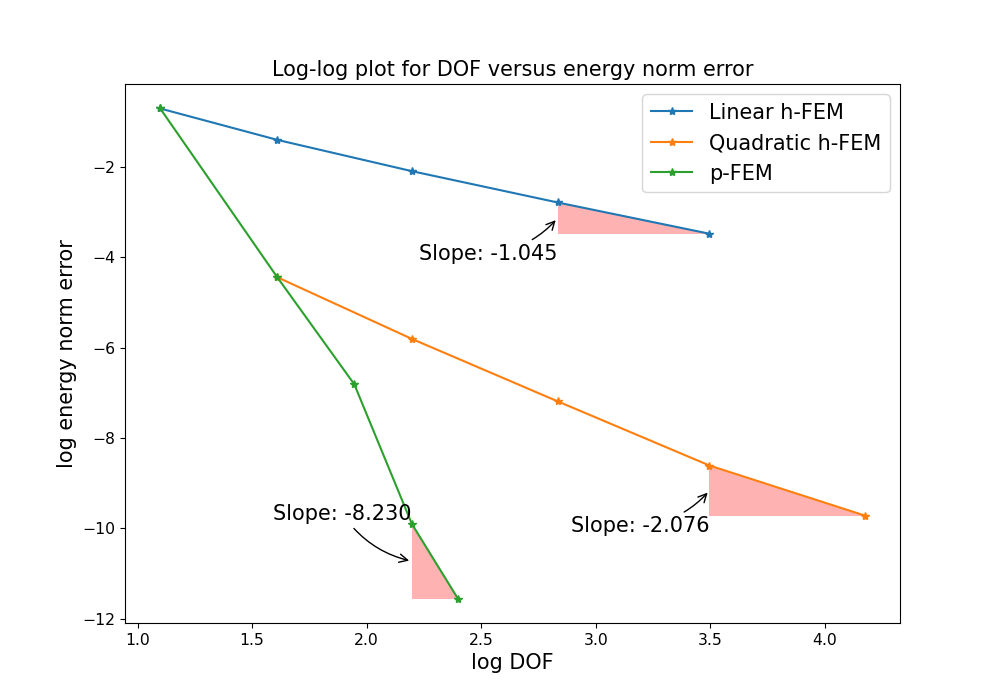
\includegraphics[width=1.\linewidth]{Q1/h_p_error.png}
  \caption{ log-log plot of the error versus DOF in h-version and p-version FEM.}
  \label{fig:h_p_error}
\end{figure}

\subsection{Question 3}

In order to estimate the error in our finite element method solutions, we use a posteriori error analysis based on the energy norms described in the following processes.

Considering the algebraic convergence of the energy norm error for exact solution $u$ and the finite elements solution $u_h$ in energy space $\epsilon(\Omega)$:

\begin{equation}
  \left\|u-u^h\right\|_{\epsilon(\Omega)} \leqslant C_1 h^{\beta_h}\|u\|_{\epsilon(\Omega)}
\end{equation}

We went:

\begin{equation}
 \|u\|_{\epsilon(\Omega)} = \sqrt{U}
\end{equation}
where $U$ is the exact energy.

Considering the relation between the energy and binary term in the finite element methods.

\begin{equation}
  \begin{aligned}
  u(u) &= \frac{1}{2} B(u, u), \\
  \|u\|_e &= \sqrt{\frac{1}{2} B(u, u)}, \\
  \|u-u^h\|_e &= \frac{1}{2} B\left(u-u^h, u-u^h\right) \\
  &= \frac{1}{2} B(u, u) - \frac{1}{2} B\left(u^h, u^h\right), \\
\end{aligned}
\end{equation}

Now we obtain the error of the strain energy:

\begin{equation}
  \begin{aligned}
U_e &= U - U^h.
\end{aligned}
\end{equation}

By using the energy values obtained from three different mesh sizes, a system of equations can be constructed to determine the exact solution 
$U$:
\begin{equation}
\begin{aligned}
  & U-U^{h_0}=C_1^2 h_0^{2 \beta_h} U \, \text{(I)}\\
  & U-U^{h_1}=C_1^2 h_1^{2 \beta_h} U \, \text{(II)}\\
  & U-U^{h_2}=C_1^2 h_2^{2 \beta_h} U \, \text{(III)}
\end{aligned}
\label{eq:U_h}
\end{equation}

In these equations:
\begin{itemize}
    \item \( U^{h_0} \), \( U^{h_1} \), and \( U^{h_2} \) are the FEM approximated solutions for mesh sizes \( h_0 \), \( h_1 \), and \( h_2 \) respectively.
    \item \( C_1 \) is a coefficient.
    \item \( \beta_h\) is an exponent that determines the convergence rate of error reduction as mesh size decreases.
\end{itemize}

The logarithmic relationship between the errors for different mesh sizes can be obtained obtained by Eq.\ref{eq:U_h}:

\begin{equation}
\begin{aligned}
  \text{Take } \frac{\log(\text{I})}{\log(\text{II})} & : \log \left( \frac{U-U^{h_0}}{U-U^{h_1}} \right) = 2 \beta_h \log \left(\frac{h_0}{h_1}\right) \\
  \text{Take } \frac{\log(\text{II})}{\log(\text{III})} & : \log \left( \frac{U-U^{h_1}}{U-U^{h_2}} \right) = 2 \beta_h \log \left(\frac{h_1}{h_2}\right) \\
\end{aligned}
\label{eq:logU_h} 
\end{equation}

These equations provide insight into how the error changes logarithmically as the mesh size changes.

Using the above relationships, the a posteriori error estimate, which is a measure of the relative error, is expressed as:

\begin{equation}
\frac{\log \left( \frac{U-U^{h_0}}{U-U^{h_1}} \right)}{\log \left( \frac{U-U^{h_1}}{U-U^{h_2}} \right)} = \frac{\log \left( \frac{h_0}{h_1} \right)}{\log \left( \frac{h_1}{h_2} \right)} = \textbf{Q}
\label{eq:Q_relation}
\end{equation}

Considering the relation between the mesh size $h$ and the $DOF$ ($N$):

\begin{equation}
 h \cong \frac{1}{N^{1 / dimensionality}}
\end{equation}

The expression of $\textbf{Q}$ is given by:

\begin{equation}
  Q=\frac{\log \left(N_1 / N_0\right)}{\log \left(N_2 / N_1\right)}
\end{equation}

The term \( \textbf{Q} \) gives a weighted comparison of the errors between different mesh sizes. This relationship becomes pivotal in understanding the error behavior across different mesh sizes.

By repeatedly applying the aforementioned process for multiple mesh sizes and averaging the computed energies, a more accurate representation of the solution's energy is achieved, which provides a reliable posterior error estimate.

\begin{table}[h]
  \centering
  \begin{tabular}{|l|c|c|}
      \hline
      & \textbf{Energy} & \textbf{Relative Error} \\
      \hline
      Linear & 0.034626674 & 2.7117($\%$) \\
      \hline
      Quadratic & 0.035591726 & 0.00132($\%$) \\
      \hline
      Exact solution & 0.035591838 & $/$ \\
      \hline
  \end{tabular}
  \caption{Energy obtained by a posterior estimate and Relative Error values for different FEM methods}
  \label{tab:fem_values}
\end{table}
Certainly, based on the table provided, here's a suitable answer:

The table.\ref{tab:fem_values} presents the energy values obtained using different Finite Element Methods (FEM) and their respective relative errors when compared to the exact solution. 

For the linear FEM, the energy is computed to be \(0.03463\), which results in a relative error of \(2.7117\%\). This indicates a slight deviation from the exact solution. On the other hand, the quadratic FEM provides an energy value of \(0.03559\), which is extremely close to the exact solution with a minuscule relative error of \(0.00132\%\). This suggests that the quadratic FEM is significantly more accurate than the linear FEM for this problem. The exact solution, as expected, has an energy of \(0.03559\) with no relative error.

In summary, while the linear FEM offers a reasonable approximation, the quadratic FEM provides an almost exact match to the true solution in terms of energy.

The code for a posterior estimate is provided in the Appendix.\ref{Apdx:post}.

\subsection{Question 4}
In the h-version study using the quadratic finite element method, we analyzed the model with varying mesh sizes, namely 5, 10, 20, and 40 evenly spaced elements. Fig.\ref{fig:q_4} represents the h-FEM solutions with four mesh sizes. A comparison of the numerical solutions against the exact solution provided insights into the accuracy of the employed method. From Fig.\ref{fig:h_error_4} it was discernible that the graph wasn't strictly linear. However, by focusing on the terminal two data points, we derived an asymptotic rate of convergence of \(-2.122\). This suggests a quadratic rate of reduction in error relative to the refinement in element size. For this specific problem, the exact strain energy is given by \( U = 1.585854059271320 \), and our computed results closely mirrored this value.  

\begin{figure}[!ht]
  \centering
  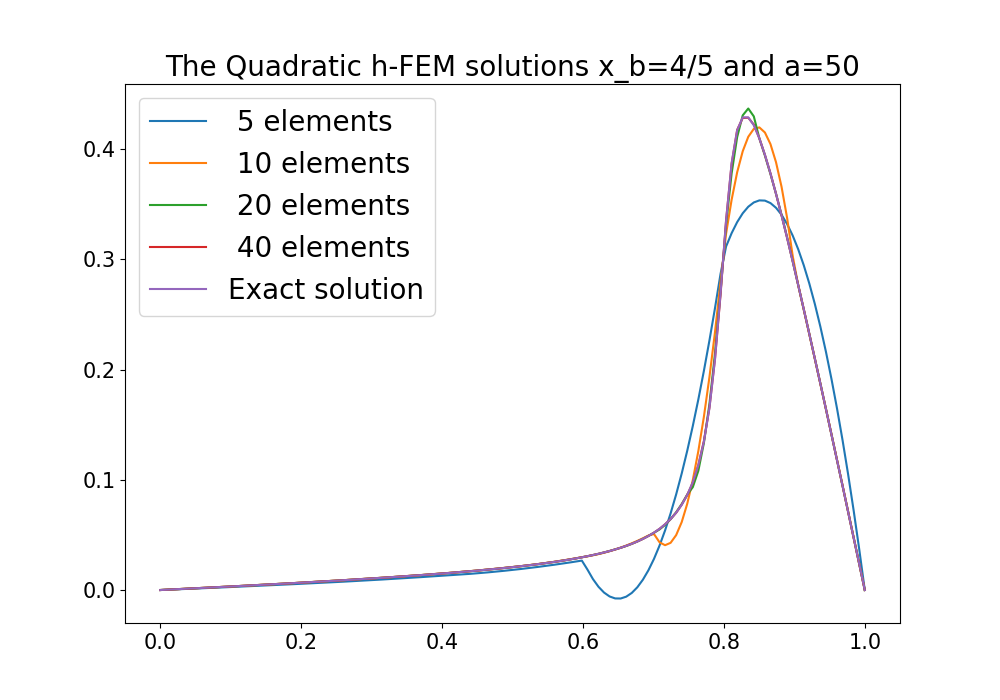
\includegraphics[width=1.\linewidth]{Q1/Q1_4.png}
  \caption{The Quadratic h-FEM solutions $x_b$=4/5 and $a$=50 with different element numbers.}
  \label{fig:q_4}
\end{figure}

\begin{figure}[!ht]
  \centering
  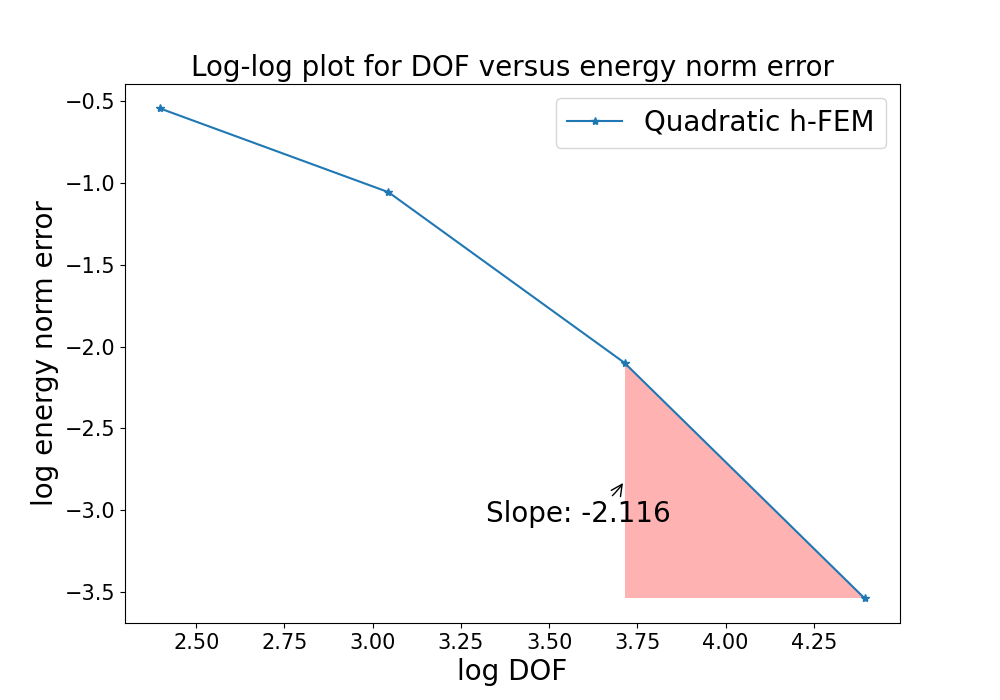
\includegraphics[width=1.\linewidth]{Q1/logDOF_q_4.png}
  \caption{Log-log plot for DOF versus energy norm error.}
  \label{fig:h_error_4}
\end{figure}

\subsection{Question 5}
In the p-version study, the problem was analyzed using 5 elements with polynomial degrees ranging from \( p = 1 \) to \( p = 5 \). The numerical solutions obtained were juxtaposed against the exact solution, providing a comprehensive understanding of the precision of our approach, as depicted in Fig.\ref{fig:p_5}. Further insights were gleaned from the log-log plot showcasing the relative error in the energy norm against the number of DOFs, illustrated in Fig.\ref{fig:h_p_error_5}. 

From the log-log plot, the computed rate of convergence for the p-version was approximately \(-0.305\), whereas for the h-version, it was \(-2.2122\). The convergence rate of quadratic h-FEM is faster than p-FEM in this problem. However, for a comparable range of DOFs (specifically from 11 to 21 DOFs), the p-version displayed a lower error than the h-version. This underscores the efficacy of the p-version in yielding more accurate results with fewer degrees of freedom.

\begin{figure}[!ht]
  \centering
  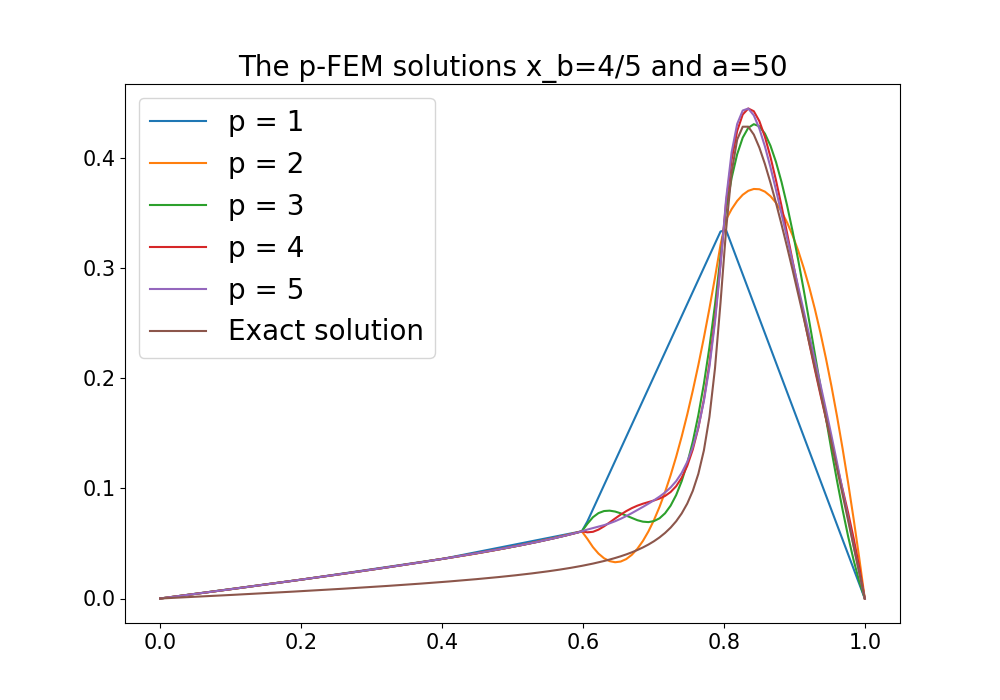
\includegraphics[width=1.\linewidth]{Q1/Q1_5.png}
  \caption{The p-FEM solutions $x_b$=4/5 and $a$=50 with different element numbers.}
  \label{fig:p_5}
\end{figure}

\begin{figure}[!ht]
  \centering
  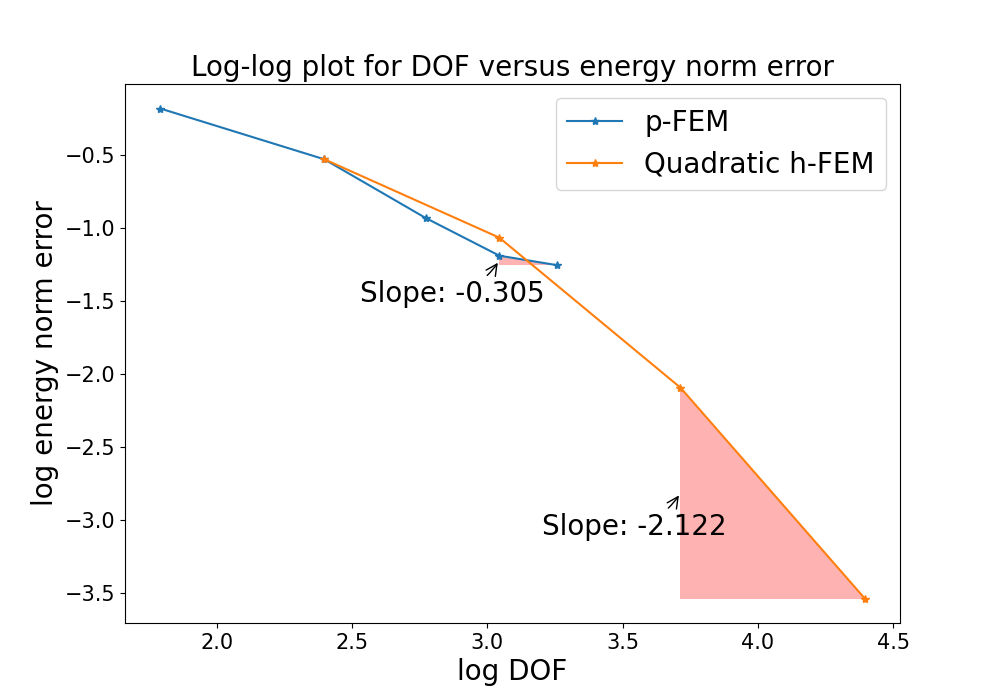
\includegraphics[width=1.\linewidth]{Q1/h_p_error_5.png}
  \caption{Log-log plot for DOF versus energy norm error in p-FEM and h-FEM.}
  \label{fig:h_p_error_5}
\end{figure}

\subsection{Question 6}
Log-log plot for the condition number of the reduced matrix $K_{ff}$ versus energy norm error for the h-FEM and p-FEM results is represented in Fig.\ref{fig:contK}.
\begin{figure}[!ht]
  \centering
  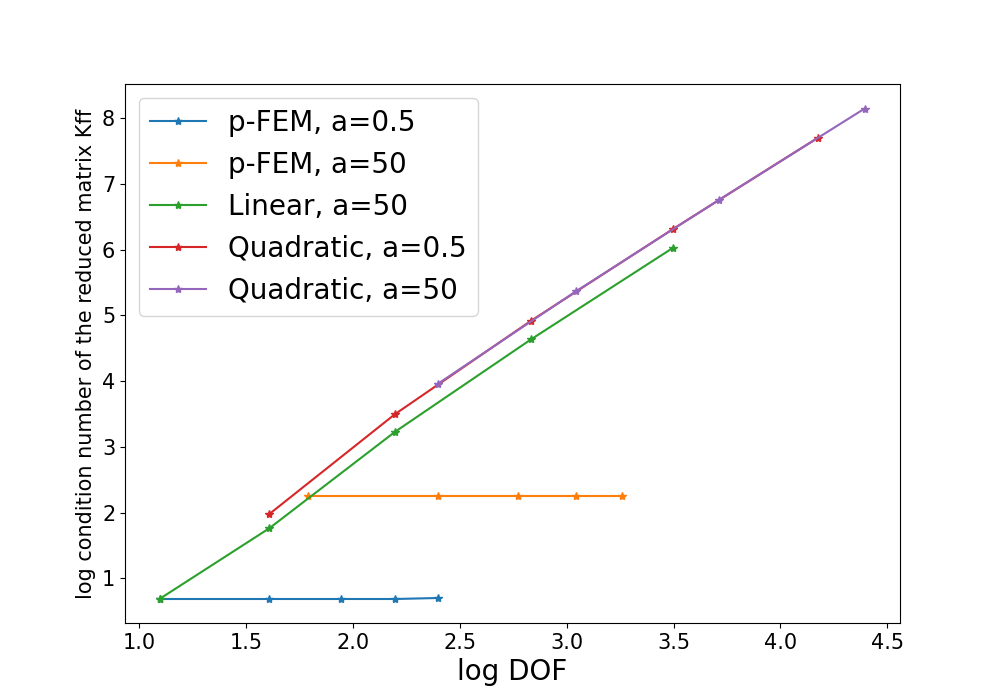
\includegraphics[width=1.\linewidth]{Q1/cont_K.png}
  \caption{Log-log plot for the condition number of the reduced matrix $K_{ff}$ versus energy norm error.}
  \label{fig:contK}
\end{figure}

\subsection{Question 7}

\subsubsection{Comparison of Results and Conclusions on Strong Gradients}
From the results obtained, several conclusions can be drawn regarding the behavior of the finite element methods under study, especially in problems with strong gradients or sharp features.

\begin{itemize}
    \item \textbf{Convergence Rate and Accuracy}: The convergence rate, represented as the slope of the log-log plot, provides insights into the efficacy of the different finite element methods. The error decreased with the increase of the DOFs and the decrease of the mesh size. Notably, the quadratic elements exhibited a more significant convergence rate than the linear ones, reflecting the theoretical expectations.
    
    \item \textbf{Linear h-version}: For the linear FEM, the energy was computed to be somewhat deviated from the exact solution, especially in problems with sharp features. This indicates that while the linear h-FEM offers a reasonable approximation, there's a clear margin for improvement in accuracy for such problems.
    
    \item \textbf{Quadratic h-version}: In sharp gradient problems, the quadratic h-FEM showed its strength by providing an energy value that was extremely close to the exact solution, emphasizing its higher accuracy.
    
    \item \textbf{p-version vs. h-version in Sharp Problems}: In problems with sharp gradients, the p-version exhibited remarkable resilience and adaptability. Despite its slower convergence rate, it outperformed both the linear and quadratic h-versions in terms of accuracy for comparable DOFs. This suggests that the p-version, with its adaptability, can better capture local variations and sharp features without requiring extensive mesh refinements that h-version methods might demand.
    
    \item \textbf{Effect of Strong Gradients}: For problems with strong gradients or sharp features, the quadratic FEM is better suited due to its adaptability and ability to capture local variations more accurately.
    
\end{itemize}

\subsubsection{Quadrature Points and Computation Efficiency}
Regarding the Gauss quadrature points, six points were chosen for the finite element computations. The rationale behind this choice was twofold. Firstly, the use of a higher number of Gauss points typically results in increased precision during integration, thus ensuring more accurate results. Secondly, given the efficiency of the computational setup, the addition of these extra points did not noticeably affect the overall computational time. As such, opting for six Gauss points struck a balance between computational efficiency and the desire for enhanced accuracy in the results.


%------------------------------------------------

\section{On \LaTeX{}}

The following is a compilation of frequently used \LaTeX{} constructs that you can use to build your report. You can find further information in the \LaTeX{} cheat sheet provided in class.

Itemized lists are given in this format:
\begin{itemize}
\item Item $1$;
\item Item $2$;
\item ...
\item Item $N$.
\end{itemize}

Enumerated lists are given in this format:
\begin{enumerate}
\item First item;
\item Second item;
\item ...
\item Last item.
\end{enumerate}

Citations can be included by using the \texttt{cite} command:~\cite{Figueredo:2009dg}. You also have to add the bibliographic entry at the end of the file.

Text requiring further explanation\footnote{Example footnote}.

\begin{figure}[!ht]
  \centering
  \includegraphics[width=1.\linewidth]{example-image-b}
  \caption{A figure that takes a single column.}
  \label{fig:label_B}
\end{figure}


Figures~\ref{fig:label_A} and \ref{fig:label_B} show, respectively, figures that take the entire width or only one columen.

\begin{figure*}
  \centering
  \includegraphics[width=6cm]{example-image-a}
  \caption{A figure that spans both columns.}
  \label{fig:label_A}
\end{figure*}

You can also add subfigures using the \texttt{subcaption} package. You can refer to the total figure with~\ref{fig:subfigures} or to individual components as~\ref{fig:subfigure_a}-\subref{fig:subfigure_c}.
\begin{figure}
  \begin{subfigure}[c]{0.32\textwidth}
    \includegraphics[width=1.\linewidth]{example-image-a}
    \caption{}
    \label{fig:subfigure_a}
  \end{subfigure}
  \begin{subfigure}[c]{0.32\textwidth}
    \includegraphics[width=1.\linewidth]{example-image-b}
    \caption{}
    \label{fig:subfigure_b}
  \end{subfigure}
  \begin{subfigure}[c]{0.32\textwidth}
    \includegraphics[width=1.\linewidth]{example-image-c}
    \caption{}
    \label{fig:subfigure_c}
  \end{subfigure}
  \caption{This is the caption for the entire figure: (a) Left; (b) Middle; and (c) Right.}
  \label{fig:subfigures}  
\end{figure} 




Here there is a complex table prepared in \LaTeX{} that showcases several improvements over standard tables, including footnotes, handling multiple hierarchical levels using \texttt{multirow} and \texttt{multicolumn}, different alignment options using custom column commands, partial rules, and coloring particular cells or even entire columns.

\ra{1.3}
\begin{threeparttable}
\begin{tabularx}
{0.5\textwidth}{X R{1} R{1} C{1}{black!5} }\toprule
&\multicolumn{3}{c}{\scell{categories}{Turquoise!25}} \\
\cmidrule{2-4} % draw rule partially
& A & B & C\tnote{\textdagger} \\ \midrule
\multirow{3}{*}{A} & 1 & 2 & 3 \\
                   & 4 & 5 & 6 \\
                   & 7 & 8 & 9 \\ \bottomrule
\end{tabularx}
\begin{tablenotes}
  \item[\textdagger]Center-aligned
\end{tablenotes}
\end{threeparttable}



Equations can be written using hte \texttt{equation} environment:
\begin{equation}
\label{eq:de-fem}
 s \vb*{v} = \vb*{T} \vb*{v} 
\end{equation}
Notice the notation for scalars, vectors, and tensors. In addition, you can use $\grad, \div$ to denote gradient and divergence. 
If you need to align equations, you can use the \texttt{align} environment:
\begin{align}
  \dd{x} && \dv{x} && \dv{f}{x} && \dv[n]{f}{x}, \label{derivatives} \\
   && \pdv{x} &&  \pdv{f}{x} && \pdv[n]{f}{x}. \label{partial}
\end{align} 
Here you also have the syntax for braces and (partial) derivatives. Equations can also be referred with~\eqref{derivatives} and~\eqref{partial}. If a single equation number is needed for an equation spanning multiple lines, use the \texttt{aligned} environment inside the \texttt{equation} environment:
\begin{equation} \label{eq:alignment}
\begin{aligned}	
  \abs{a} && \norm{b},  \\
     \qty(a) && \qty[b] && \qty{c} && \qty|d|,
\end{aligned}
\end{equation}
where you see the syntax used for braces.


Some results will require log-log plots, which can be created in \LaTeX{} using the \texttt{pgfplots} package:
\begin{figure}
\pgfplotsset{
    cycle list/Dark2,
    cycle multiindex* list={
        mark list\nextlist
        Dark2\nextlist
    },
}
\centering
\begin{tikzpicture}[]       

  \begin{loglogaxis}[
    scale only axis=true,
    width = 5 cm, height = 5cm,
    xlabel near ticks, ylabel near ticks,
    xlabel=$x$,
    ylabel=$y \left( x \right)$,
    legend style={at={(1,1)}, anchor=north east, draw=none, fill=none},
  ]

    \addplot+ [dashed, domain=10:1000] { 10/x) };
    \addlegendentry{legend 1}
    
    \addplot+ [ultra thick, dotted] table[]{
      10  0.5 10
      100  0.1 20
      1000  0.05 30
    }
    coordinate [pos=0.15] (A)
    coordinate [pos=0.25] (B)
    coordinate [pos=0.25] (C);
    \addlegendentry{legend 1}
    \coordinate (A') at ($(A)!3pt!90:(B)$);
    \coordinate (B') at ($(B)!3pt!270:(A)$);
    \draw  (A') -| (B') node[pos=0.25,above]{\small $1$} node[pos=0.75,right]{$\alpha$};
    \draw [shorten <=-3pt,shorten >=-3pt] (A') -- (B');
  \end{loglogaxis}
\end{tikzpicture}
\caption{A log-log plot.}
\end{figure}


%------------------------------------------------

\section{Discussion}

The discussion is a very important part of the report, so make sure you write it properly.

%----------------------------------------------------------------------------------------
%	REFERENCE LIST
%----------------------------------------------------------------------------------------

% \begin{thebibliography}{99} % Bibliography - this is intentionally simple in this template

% \bibitem[Figueredo and Wolf, 2009]{Figueredo:2009dg}
% Figueredo, A.~J. and Wolf, P. S.~A. (2009).
% \newblock Assortative pairing and life history strategy - a cross-cultural
%   study.
% \newblock {\em Human Nature}, 20:317--330.
 
% \end{thebibliography}

%----------------------------------------------------------------------------------------


\Large{Remember there is a 10-page limit!}
\hrule 
%%\newpage
%%\bibliographystyle{apacite}
%%\bibliography{sample}
\bibliographystyle{plain} % or another suitable bibliography style
\bibliography{ref.bib} % the name of your .bib file without the extension
% Start the appendix
\appendix
\section{Finite elements methods in 1-D main codes}
\label{Apdx:FEM_1D}
\begin{lstlisting}[language=Python, caption=Finite elements methods in 1-D main code]
  def FEM_1D(shape_class = Hierarchical, p = 3, num_elems = 3, domain = (0, 1),rhs_func = rhs_fn(a=50, xb=0.8), exact_func=exact_fn(0.5,0.8), BCs = (0, 0), verbose = False):
      N=6
      mesh = np.linspace(domain[0], domain[1], num_elems+1)
      ori_phi_phip = {'phis': [], 'phips': []}
      for elem in range(num_elems):
          scale = [mesh[elem], mesh[elem+1]]
          phis, phips = shape_class(scale, p)
          ori_phi_phip['phis'].append(phis)
          ori_phi_phip['phips'].append(phips)
  
  
      linear_phi_phip = {'phis': [], 'phips': []}  # Linear
      for elem in range(num_elems):
          linear_phis = []
          linear_phips = []
          for idx in range(len(ori_phi_phip['phis'][elem])):
              if ori_phi_phip['phis'][elem][idx].p < 2:
                  phi = ori_phi_phip['phis'][elem][idx]
                  phip = ori_phi_phip['phips'][elem][idx]
                  linear_phi_phip['phis'].append(phi)
                  linear_phi_phip['phips'].append(phip)
                  linear_phis.append(phi)
                  linear_phips.append(phip)
          linear_K_sub = np.zeros((len(linear_phips), len(linear_phips)))
          for indx, x in np.ndenumerate(linear_K_sub):
              linear_K_sub[indx] = G_integrate(
                  mul(linear_phips[indx[0]], linear_phips[indx[-1]]), N=6, scale=linear_phips[indx[0]].scale)
              if abs(linear_K_sub[indx]) < 1e-10:
                  linear_K_sub[indx] = 0
          linear_F_sub = np.zeros(len(linear_K_sub))
          for indx in range(len(linear_F_sub)):
              linear_F_sub[indx] = G_integrate(
                  mul(rhs_func, linear_phis[indx]), N=N, scale=linear_phis[indx].scale)
          if elem == 0:
              K = linear_K_sub
              F = linear_F_sub
          else:
              K = assemble(K, linear_K_sub)
              F = assemble(F, linear_F_sub)
              
      linear_num = len(F)
  
      nonlinear_phi_phip = {'phis': [], 'phips': []}
      for order in range(2, p+1):  # Non Linear
          for elem in range(num_elems):
              for idx in range(len(ori_phi_phip['phis'][elem])):
                  if (ori_phi_phip['phis'][elem][idx].p == order) or (ori_phi_phip['phips'][elem][idx].p == order):
                      nonlinear_phi = ori_phi_phip['phis'][elem][idx]
                      nonlinear_phip = ori_phi_phip['phips'][elem][idx]
                      nonlinear_phi_phip['phis'].append(nonlinear_phi)
                      nonlinear_phi_phip['phips'].append(nonlinear_phip)
                      nonlinear_K_sub = np.zeros((2, 2))
                      
                      nonlinear_K_sub[-1, -1] = G_integrate(mul(nonlinear_phip, nonlinear_phip),N=N, scale=nonlinear_phip.scale)
                      nonlinear_F_sub = np.zeros(2)
                      nonlinear_F_sub[-1] = G_integrate(mul(rhs_func, nonlinear_phi), N=N, scale=nonlinear_phi.scale)
  
                      K = assemble(K, nonlinear_K_sub)
                      F = assemble(F, nonlinear_F_sub)
                  else:
                      pass
                  
      # Applying boundary condition
  
      K[0, 1:] = 0.0 
      K[linear_num-1, :linear_num-1] = 0.0
      F[0] = BCs[0]* K[0, 0] 
      F[linear_num-1] = BCs[-1] * K[linear_num-1, linear_num-1]
  
      U = -la.solve(K, F)
      phi_phip = {'phis': [], 'phips': []}
      phi_phip['phis'] = joint_funcs(linear_phi_phip['phis']) + nonlinear_phi_phip['phis']
      phi_phip['phips'] = joint_funcs(linear_phi_phip['phips']) + nonlinear_phi_phip['phips']
      u_list = []
      for i in range(len(phi_phip['phis'])):
          u_list.append(mul(U[i], phi_phip['phis'][i]))
      uh = plus(u_list)
      if verbose == True:
          print(f"Shape class: {shape_class.__name__}, Number of elements: {num_elems}, Polynomial order:{p},  Domain: {domain}, Boundary conditions: {BCs}")
          x_data = np.linspace(domain[0], domain[1], 101)
          plt.plot(x_data, exact_func(x_data), label='Analytical solution')
          plt.plot(x_data, uh(x_data), label='FEM solution {} elements'.format(num_elems))
          for i in range(len(phi_phip['phis'])):
              func = phi_phip['phis'][i]
              plt.plot(x_data, U[i]*func(x_data))
          plt.legend()
          plt.show()
      eigenvalues = np.linalg.eigvals(K)
      cont_K = max(eigenvalues)/min(eigenvalues)
      return U, phi_phip, uh, cont_K
  
\end{lstlisting}

\section{Defeinition of the shape functions in 1-D}
\label{Apdx:shape_1D}
\begin{lstlisting}[language=Python, caption=Defeinition of the shape functions in 1-D]
def Legendre(x=np.linspace(-1, 1, 100), p=5):

  if p == 0:
      return 1
  elif p == 1:
      return x

  else:
      return ((2*p-1)*x*Legendre(x, p-1)+(1-p)*Legendre(x, p-2))/p

class shape_function:
      def __init__(self, scale=[-1, 1]):
          self.scale = scale
          self.x_l = scale[0]
          self.x_r = scale[1]
          self.range = [-1, 1]
          
      def expression(self, x):
          return 1 - (x - self.x_l) / (self.x_r - self.x_l)
      
      def mapping(self, x):
          scale = self.scale
          range = self.range
          x_normalized = (x - scale[0]) / (scale[1] - scale[0])
          return range[0] + x_normalized * (range[1] - range[0])
  
      def __call__(self, x):
          x = np.asarray(x)  # convert x to a numpy array if it's not already
          expression_vectorized = np.vectorize(self.expression, otypes=['d'])
          return np.where((self.scale[0] <= x) & (x <= self.scale[-1]), expression_vectorized(x), 0)
      
class phi_func_l(shape_function):
  def __init__(self, scale, p):
      super().__init__(scale)
      self.p = p
      self.range = [0, 1]
  def expression(self, x):
      if self.p == 0:
          phi = 1-self.mapping(x)
      elif self.p == 1:
          phi = self.mapping(x) 
      else:
          raise AssertionError("p should be 0 or 1 in linear shape function, not{}".format(self.p))
      return phi
      
class phip_func_l(shape_function):
  def __init__(self, scale, p):
      super().__init__(scale)
      self.range = [0, 1]
      self.p = p
  def expression(self, x):
      scale_up = 1/(self.scale[1]-self.scale[0]) 
      
      if self.p == 0:
          phip =  np.zeros_like(self.mapping(x))-1
      elif self.p == 1:
          phip = np.zeros_like(self.mapping(x))+1
      else:
          raise AssertionError("p should be 0 or 1 in linear shape function, not{}".format(self.p))
      return phip*scale_up
  
class phi_func_q(shape_function):
  def __init__(self, scale, p):
      super().__init__(scale)
      self.range = [0, 1]
      self.p = p
  def expression(self, x):
      xx = self.mapping(x)
      if self.p == -1:
          phi = (xx-1)*(xx-0.5)*2
      elif self.p == 0:
          phi = -xx*(xx-1)*4
      elif self.p ==1:
          phi = xx*(xx-0.5)*2
      else:
          raise AssertionError("p should be -1, 0 or 1 in quadratic shape function, not{}".format(self.p))
      return phi
      
class phip_func_q(shape_function):
  def __init__(self, scale, p):
      super().__init__(scale)
      self.range = [0, 1]
      self.p = p
  def expression(self, x):
      scale_up = 1/(self.scale[1]-self.scale[0]) 
      xx = self.mapping(x)
      if self.p == -1:
          phip = 4*xx - 3.0
      elif self.p == 0:
          phip = 4-8*xx
      elif self.p ==1:
          phip = 4*xx - 1.0
      else:
          raise AssertionError("p should be -1, 0 or 1 in quadratic shape function, not{}".format(self.p))
      return phip*scale_up
  
class phi_func_h(shape_function):
  def __init__(self, scale, p):
      super().__init__(scale)
      self.p = p
  def expression(self, x):
      scale = self.scale
      i =self.p
      if i == 0:
          phi = (1-self.mapping(x))/2 
      elif i == 1:
          phi = (1+self.mapping(x))/2 
      else:
          phi = 1/np.sqrt(4*i-2)*(Legendre(self.mapping(x), i)-Legendre(self.mapping(x), i-2))
      return phi
      
class phip_func_h(shape_function):
  def __init__(self, scale, p):
      super().__init__(scale)
      self.p = p
  def expression(self, x):
      scale_up = 2/(self.scale[1]-self.scale[0]) 
      i =self.p
      
      if i == 0:
          phip =  np.zeros_like(self.mapping(x))-0.5
      elif i == 1:
          phip = np.zeros_like(self.mapping(x))+0.5
      else:
          phip = np.sqrt(i-1/2)*(Legendre(self.mapping(x), i-1))
      return phip*scale_up
  
def Hierarchical(scale, p):
  phis = []
  phips = []
  start=0
  
  for i in range(start, p+1):
      new_phi = phi_func_h(scale, i)
      new_phip = phip_func_h(scale,i)
      phis.append(new_phi)
      phips.append(new_phip)
  return phis, phips

def linear(scale, p):
  phis = []
  phips = []
  p = 1
  for i in range(p+1):
      new_phi = phi_func_l(scale, i)
      new_phip = phip_func_l(scale,i)
      phis.append(new_phi)
      phips.append(new_phip)
  return phis, phips

def quadratic(scale, p):
  phis = []
  phips = []
  p = 1
  for i in range(-1, p+1):
      new_phi = phi_func_q(scale, i)
      new_phip = phip_func_q(scale,i)
      phis.append(new_phi)
      phips.append(new_phip)
  return phis, phips
\end{lstlisting}

\section{Defeinition of Gaussian integrate in 1D}
\label{Apdx:Gaussian-1D}
\begin{lstlisting}[language=Python, caption=Defeinition of Gaussian integrate in 1D]
def G_integrate(u, N=3, scale=(0, 1)):
  N = N  
  a = scale[0] 
  b = scale[1]
  x, w = roots_legendre(N)

  xp = x*(b-a)/2+(b+a)/2
  wp = w*(b-a)/2

  s = 0
  for i in range(N):
      s += wp[i]*u(xp[i])
  return s
\end{lstlisting}
  

\section{A posteriori error estimate}
\label{Apdx:post}
\begin{lstlisting}[language=Python, caption=A posteriori error estimate]
def posterior_energy(energy_list_array, DOFs_array):
  if len(energy_list_array)<3:
      raise AssertionError("The value of energy should be greater than three!")
  elif len(energy_list_array)!= len(DOFs_array):
      raise AssertionError("The number of energy values should be equal to the number of DOFs!")
  def equation(U, U0, U1, U2, Q):
      return ((U-U0)/(U-U1) / ((U-U1)/(U-U2))**Q - 1)**2

  i = 0
  U_list = []
  while i+3 <= len(energy_list_array):
      U0, U1, U2 = energy_list_array[i:i+3]
      h0, h1, h2 = 1/np.sqrt(DOFs_array[i:i+3])
      # print(h0, h1, h2)
      N0, N1, N2 = DOFs_array[i:i+3]
      # Q = np.log((h0/h1))/np.log((h1/h2))
      Q = np.log((N1/N0))/np.log((N2/N1))
      initial_guess = np.mean(energy_list_array)
      # Use minimize
      U_solution = minimize(equation, initial_guess, args=(U0, U1, U2, Q)).x
      U_list.append(U_solution )
      i+=1
return np.mean(U_list)
\end{lstlisting}
  

















 
\end{document}
